%iffalse
\let\negmedspace\undefined
\let\negthickspace\undefined
\documentclass[journal,12pt,onecolumn]{IEEEtran}
\usepackage{cite}
\usepackage{amsmath,amssymb,amsfonts,amsthm}
\usepackage{algorithmic}
\usepackage{graphicx}
\usepackage{textcomp}
\usepackage{xcolor}
\usepackage{txfonts}
\usepackage{listings}
\usepackage{enumitem}
\usepackage{mathtools}
\usepackage{gensymb}
\usepackage{comment}
\usepackage[breaklinks=true]{hyperref}
\usepackage{tkz-euclide} 
\usepackage{listings}
\usepackage{gvv}                                        
\def\inputGnumericTable{}                                 
\usepackage[latin1]{inputenc}                                
\usepackage{color}                                            
\usepackage{array}                                             
\usepackage{longtable}                                       
\usepackage{calc}                                             
\usepackage{multirow}                                         
\usepackage{hhline}                                           
\usepackage{ifthen}                                           
\usepackage{lscape}
\usepackage{multicol}

\newtheorem{theorem}{Theorem}[section]
\newtheorem{problem}{Problem}
\newtheorem{proposition}{Proposition}[section]
\newtheorem{lemma}{Lemma}[section]
\newtheorem{corollary}[theorem]{Corollary}
\newtheorem{example}{Example}[section]
\newtheorem{definition}[problem]{Definition}
\newcommand{\BEQA}{\begin{eqnarray}}
\newcommand{\EEQA}{\end{eqnarray}}
\newcommand{\define}{\stackrel{\triangle}{=}}
\theoremstyle{remark}
\newtheorem{rem}{Remark}
\begin{document}

\bibliographystyle{IEEEtran}
\vspace{3cm}

\title{NCERT - 8.3.17}
\author{EE224BTECH11044 - Muthyala koushik
}
\maketitle
\bigskip

\renewcommand{\thefigure}{\theenumi}
\renewcommand{\thetable}{\theenumi}
\textbf{\section{APPLICATION OF INTEGRALS}}

\textbf{Question:} The area bounded by the curve $y=x\abs{x}$, $x$-axis and the ordinates $x = - 1$ and $x = 1$ is given by \\ 

\solution $y = x^2$ if $x > 0$ and $y = - x^2$ if $x < 0$

\begin{align}
	\text{Area}\brak{A}=\int_{-1}^{1} \abs{y} dx\\
\end{align}

Split the integral at $x=0$, as the function changes;

\begin{align}
	A&=\int_{-1}^{0} \brak{-x^2} dx+\int_{0}^{1} x^2 dx\\
	A&=-\int_{-1}^{0} \brak{-x^2} dx+\int_{0}^{1} x^2 dx\\
	A&=-\sbrak{\frac{x^3}{3}}_{-1}^{0}+\sbrak{\frac{x^3}{3}}_{0}^{1}\\
	A&=-\brak{0-\brak{-\frac{\brak{-1}^3}{3}}}+\brak{\frac{1}{3}-0}\\
	A&=\frac{1}{3}+\frac{1}{3}\\
	A&=\frac{2}{3}\\
	A&=0.66666666667
\end{align}

\textbf{Computational Solution:} \\
Using the trapezoidal rule,
\begin{align}
	J &= \int_a^b f\brak{x}\, dx \approx h\brak{\frac{1}{2}f\brak{a} + f\brak{x_1} + f\brak{x_2} \cdots + f\brak{x_{n-1}} + \frac{1}{2}f\brak{b}}\\
	h &= \frac{b-a}{n}\\
	A &= A_n, \text{ where, } A_{i + 1} = A_i + h\frac{f\brak{x_{n+1}} + f\brak{x_n}}{2}\\ 
	A_{i + 1} &= A_i + \frac{h}{2}\brak{ f\brak{x_{n+1}} + f\brak{x_n}}\\
	A_{i + 1} &= A_i +\frac{h}{2}\brak{ {x_{n+1}}^2 + {x_n}^2}\\ 
	x_{n+1} &= x_n + h	
\end{align}

\textbf{Initial Conditions:}
\begin{itemize}
    \item $a = -1$
    \item $b = 1$
    \item $A_0 = 0$
    \item $h = \frac{2}{n}$ (depending on the chosen number of subintervals $n$)
    \item Here we assume $n = 1000$.
\end{itemize}

$ \implies$ The theoritical value of Area is $0.66666666667$.\\
$ \implies$ The computational value of Area is $0.6666679999999998$.\\

\begin{figure}[h]
	\centering
	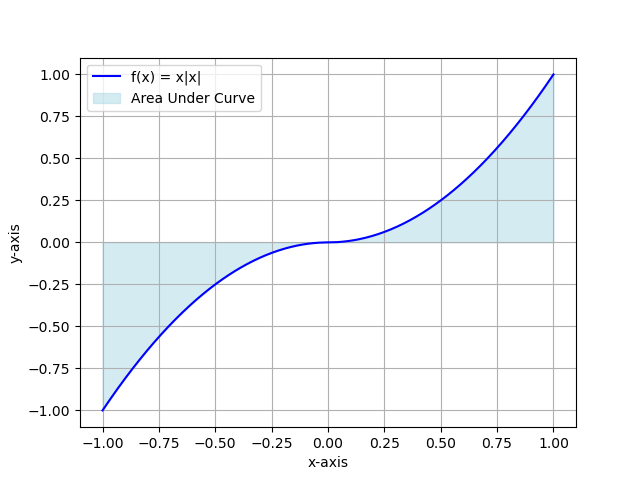
\includegraphics[width=\columnwidth]{figs/fig.png}
\end{figure}

\end{document}
